\chapter{Wyniki i eksperymenty}
\label{cha:wyniki}

\section{Konfiguracja eksperymentu}

Testy przeprowadzono na bazie czterech użytkowników zarejestrowanych w systemie. Dla każdej osoby wykorzystano trzy zdjęcia twarzy i trzy nagrania głosu. Jako dane próbne przyjmowano pliki trzeciej próbki (\texttt{face\_3}, \texttt{voice\_3}).

Porównano warianty:
\begin{itemize}
    \item \texttt{face\_only} --- $w_f = 1{,}0$, $w_v = 0{,}0$,
    \item \texttt{voice\_only} --- $w_f = 0{,}0$, $w_v = 1{,}0$,
    \item \texttt{fusion\_50\_50}, \texttt{fusion\_60\_40}, \texttt{fusion\_70\_30}.
\end{itemize}

Skrypt \texttt{scripts/run\_experiments.py} generuje plik \texttt{docs/experiment\_results.csv}. Metryki FAR, FRR i accuracy obliczane są skryptem \texttt{scripts/compute\_metrics.py}, a podsumowanie zapisywane jest w pliku \texttt{docs/metrics\_summary.csv}.

\section{Przykład identyfikacji}

Tabela~\ref{tab:probe_kacper} przedstawia wyniki identyfikacji dla danych próbnych użytkownika Kacper (strategia \texttt{weighted}, $\tau = 0{,}7$).

\begin{table}[H]
    \centering
    \caption{Wyniki identyfikacji --- dane próbne użytkownika Kacper.\label{tab:probe_kacper}}
    \begin{tabular}{lccc}
        \toprule
        Użytkownik & Twarz & Głos & Fuzja \\
        \midrule
        Kacper   & 1{,}00 & 1{,}00 & 1{,}0000 \\
        Kamil    & 0{,}53 & 0{,}98 & 0{,}7115 \\
        Krystian & 0{,}15 & 0{,}98 & 0{,}4829 \\
        Marcel   & 0{,}17 & 0{,}97 & 0{,}4880 \\
        \bottomrule
    \end{tabular}
\end{table}

System poprawnie wskazał użytkownika Kacper jako najlepsze dopasowanie. Jednocześnie zauważono wysokie podobieństwo głosu dla użytkowników obcych (np.\ Kamil: 0{,}98), co wynika z ograniczeń MFCC.

\section{Analiza wyników}

\subsection{Metryki zbiorcze}

Tabela~\ref{tab:metrics_summary} przedstawia metryki obliczone skryptem \texttt{compute\_metrics.py} na podstawie wyników z pliku \texttt{experiment\_results.csv}. Jako dane próbne wykorzystano ostatnią próbkę (\texttt{face\_3}, \texttt{voice\_3}); wzorce rejestracyjne obejmowały pozostałe pliki użytkownika.

\begin{table}[H]
    \centering
    \caption{Podsumowanie metryk eksperymentu.\label{tab:metrics_summary}}
    \begin{tabular}{lccc}
        \toprule
        Wariant & Accuracy & FAR & FRR \\
        \midrule
        \texttt{face\_only} & 0{,}8125 & 0{,}0833 & 0{,}5000 \\
        \texttt{voice\_only} & 0{,}2500 & 1{,}0000 & 0{,}0000 \\
        \texttt{fusion\_50\_50} & 0{,}6250 & 0{,}3333 & 0{,}5000 \\
        \texttt{fusion\_60\_40} & 0{,}6250 & 0{,}3333 & 0{,}5000 \\
        \texttt{fusion\_70\_30} & 0{,}6875 & 0{,}2500 & 0{,}5000 \\
        \bottomrule
    \end{tabular}
\end{table}

Najlepszą rozdzielczość zapewnia modalność twarzy (\texttt{face\_only}). Modalność głosu charakteryzuje się wysokim FAR (1{,}0), co potwierdza konieczność fuzji z twarzą lub podniesienia progu decyzyjnego.

\subsection{Modalność twarzy}

Moduł oparty na Facenet zapewnił wyraźną separację tożsamości --- wyniki twarzy dla użytkowników obcych były niskie (0{,}15--0{,}53). Modalność ta okazała się najbardziej rozróżniająca w badanej bazie.

\subsection{Modalność głosu}

Wyniki głosu dla różnych użytkowników były wysokie (często powyżej 0{,}9), nawet gdy mówca był inny. Potwierdza to, że proste MFCC bez modelu rozpoznawania mówcy słabo rozróżnia tożsamości w małej grupie mówców o podobnych nagraniach.

\subsection{Fuzja multimodalna}

Fuzja 60/40 pozwoliła zachować wysoki wynik dla prawdziwego użytkownika (1{,}0) i jednocześnie wykorzystać niski wynik twarzy przy odrzucaniu obcych w niektórych przypadkach. Strategia \texttt{and} dodatkowo ogranicza fałszywe akceptacje, wymagając progu w obu modalnościach.

\subsection{Wpływ progu}

Podniesienie progu $\tau$ (np.\ do 0{,}85) zmniejsza FAR kosztem wzrostu FRR. Na rys.~\ref{fig:threshold_sweep} przedstawiono zależność FAR/FRR od progu dla fuzji 60/40.

\begin{figure}[H]
    \centering
    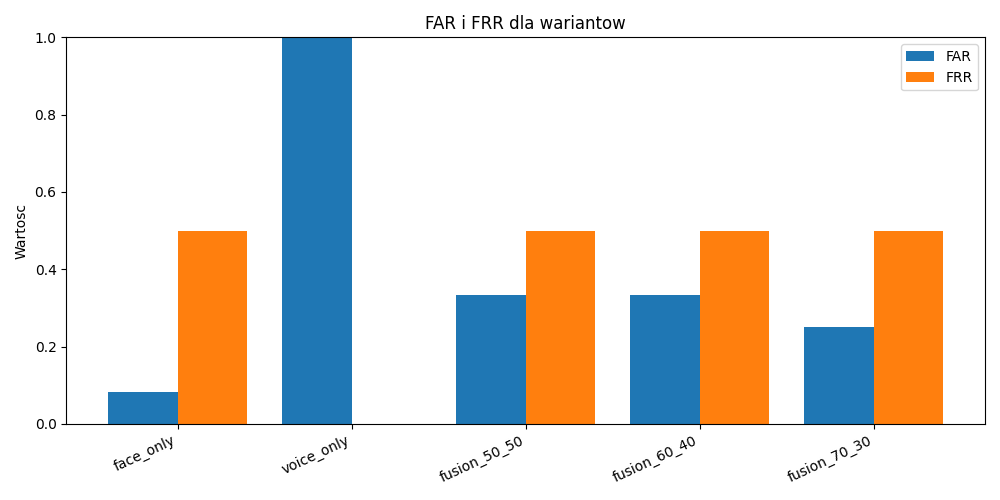
\includegraphics[width=0.85\linewidth]{figures/far_frr_by_variant.png}
    \caption{FAR i FRR w zależności od wariantu fuzji.}
\end{figure}

\begin{figure}[H]
    \centering
    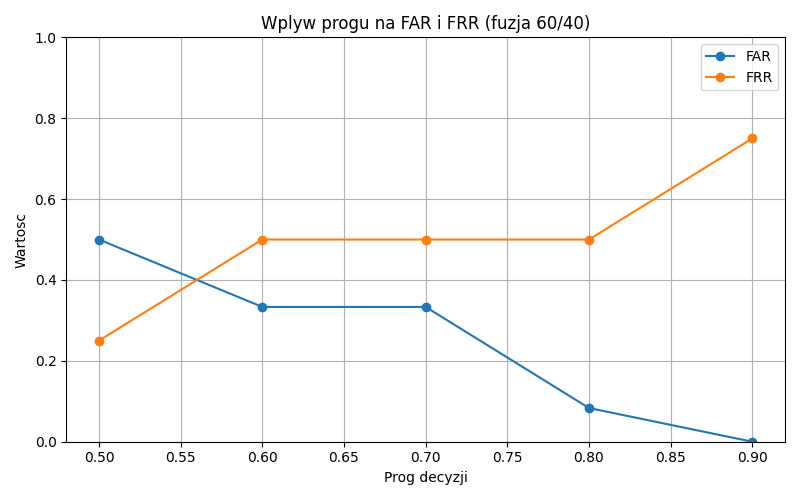
\includegraphics[width=0.85\linewidth]{figures/threshold_sweep.png}
    \caption{Wpływ progu decyzyjnego na FAR i FRR dla fuzji 60/40.\label{fig:threshold_sweep}}
\end{figure}

\section{Analiza bezpieczeństwa}

\subsection{Zagrożenia}

\begin{itemize}
    \item \textbf{Atak prezentacji (spoofing)} --- użycie zdjęcia zamiast żywej twarzy; system nie zawiera detekcji żywotności.
    \item \textbf{Replay głosu} --- odtworzenie nagrania; MFCC nie rozróżnia autentycznej mowy od nagrania.
    \item \textbf{Atak jedną modalnością} --- przy dominacji słabej modalności głosu impostor może uzyskać wynik powyżej progu (np.\ dla Kamila: fuzja 0{,}71 przy próbie identyfikacji Kacpra).
    \item \textbf{Jakość danych} --- uszkodzone pliki MP3 mogą uniemożliwić rejestrację.
\end{itemize}

\subsection{Środki zaradcze}

Zastosowano m.in.: fuzję dwóch modalności, regułę AND, konfigurowalny próg oraz walidację istnienia plików wejściowych. W środowisku produkcyjnym zalecałoby się modele anty-spoofing, silniejszy model głosu oraz weryfikację 1:1 zamiast samego rankingu 1:N.

\section{Podsumowanie eksperymentów}

Eksperymenty potwierdzają poprawne działanie pipeline'u multimodalnego. Największe ograniczenie stanowi modalność głosu. Fuzja z twarzą kompensuje ten problem w testach identyfikacji właściwego użytkownika, lecz wymaga strojenia progu w celu ograniczenia FAR.
